\section{Anwendung des Kalman-Filters}
\subsection{Ziel}
Bis jetzt haben wir gelesen, was das Kalman-Filter bewirkt und wie es funktioniert.
Nun möchten wir mit einem Beispiel herausfinden, ob das Filter unsere gesuchte Grösse $f(t)$ bestimmen kann.

\subsection{Künstliche Erdbebendaten}
Da wir keine Rohdaten über vergangene Erdbeben zur Hand haben, müssen wir mittels Matlab künstliche Daten  erzeugen und sie dann in das Filter eingeben.
Diese Vorgehensweise erlaubt uns das Erdbeben beliebig zu gestalten
und weil es digital simuliert wird, haben wir keine Bauschäden zu beklagen.

\subsection{Wahl der Schwingung}
Wir müssen uns überlegen, mit welcher Schwingung wir ein realitätsnahes Beben erzeugen können.
Mit einer ungedämpften harmonischen Schwingung können wir zwar die meisten Vorgänge in der Physik erklären.
Da aber unser Erdbeben irgendwann abklingen muss, wählen wir die gedämpfte harmonische Schwingung.
Die dazugehörige Schwingungsgleichung lautet
\begin{equation}
	y = A e^{-\lambda t} \sin(\omega t).
\end{equation}
Dabei ist $A=5$ die anfängliche Amplitude der Schwingung,
die uns die Heftigkeit des Erdebebens beschreibt.
Sie ist vergleichbar mit der Magnitude.
$\lambda$ bezeichnet die Bodendämpfung, für die wir $0.2$ wählen.
Sie ist dafür verantwortlich, dass unser Erdbeben abklingt
und kreiert die bei gedämpften Schwingungen typische Hüllkurve.
Wir nehmen an, dass $\lambda$ ein Materialparameter von geologischen Böden ist.
Die Kreisfrequenz $\omega$ ist durch
\begin{equation}
	\omega = 2 \pi f
\end{equation}
gegeben, 
wobei die Momentanfrequenz $f = \mathcal N(\mu_f, \sigma_f) $ einer Normalverteilung mit
\begin{equation}
  \mu_f = \SI{15}{\hertz}
  \qquad \text{und} \qquad
  \sigma_f = \SI{10}{\hertz}
\end{equation}
folgt.

Zusätzlich haben wir $f$ mit einem Savitzky-Golay-Filter gefiltert.
Das Savitzky-Golay-Filter schaut sich immer eine definierte Anzahl von Datenpunkte an
und bildet  darüber ein Polynom $n$-ter Ordnung.
In unserer Anwendung schaut sich das Filter, im Sinne eines verschiebbaren Fensters,
jeweils elf aufeinanderfolgende Datenpunkte an
und approximiert diese mit ein Polynom $0$-ter Ordnung,
also einer Konstanten.
Somit erhalten wir mit Matlab-Standardfunktionen einen gleitenden Mittelwert.

\subsection{Versuch im Standardfall}
Im nächsten Schritt müssen wir sinnvolle Systemparameter für unseren Seismographen definieren.
Eine kurze Recherche zeigt, dass die Masse ein Gewicht von ca.\ \SI{100}{\gram} hat.
Zur Federkonstante D und Dämpfung k konnten wir leider keine brauchbaren Grössen finden und treffen die Annahme, dass $D = 1$ und $k = 0.01$.
Für die Masse definieren wir $m = 0.01$.

Da unser Seismograph von der Umgebung durch Wind, Temperatur oder menschgemachten Vibrationen beeinflusst wird, müssen wir ein Prozessrauschen definieren.
Die dazugehörige Matrix $Q$ beinhaltet die Standardabweichung für die Position, Geschwindigkeit und äussere Kraft.
Wir nehmen an, dass

\begin{equation}
	Q = \left(
	\begin{array}{ccc}
		{\sigma_x }^2& 0& 0 \\
		0 & {\sigma_v }^2& 0\\
		0 & 0& {\sigma_f }^2\\
	\end{array}\right)= \left(
	\begin{array}{ccc}
		{0.00001}^2& 0& 0 \\
		0 & {0.00001}^2& 0\\
		0 & 0& {1 }^2\\
	\end{array}\right).
\end{equation}

Auch für die Messung setzen wir ein Rauschen voraus und definieren

\begin{equation}
R= ({\sigma_x}^2)=
({0.00001}^2).
\end{equation}

Sind nun die benötigten Systemparameter und das Rauschen definiert, erzeugen wir das Erdbeben und schauen, wie gut das Kalman-Filter die äussere Beschleunigung schätzen kann.

\subsection*{Ergebnis}

Wie wir in Abbildung~\ref{erdbeben:fig:standard-alles} im Positions-Zeit-Diagramm sehen, erzeugen unsere vorher gewählten Parameter eine realistische Erdbebenaufzeichnung.
Leiten wir die Position einmal ab, erhalten wir die Geschwindigkeit.
Die zweite Ableitung ergibt uns die Kraft, die in unserer Aufgabenstellung gesucht ist.

Zoomen wir näher ran, erkennen wir in der Abbildung~\ref{erdbeben:fig:standard-zoom} im Positions-Diagramm eine Überlagerung der Massen-Eigenschwingung mit der Erdbebenschwingung.
Die Masse schwingt mit einer tiefer Frequenz und hoher Amplitude, hingegen das Erdbeben mit einer hohen Frequenz und tiefer Amplitude.

Vergleichen wir nun die Position mit der Kraft, stellen wir fest, dass das Kalman-Filter eine Schätzung wiedergibt, die auch eine Frequenz von \SI{15}{\hertz} hat.
Das Filter war imstande die Eigenfrequenz zu eliminieren und die tatsächliche Kraft des Erdbebens zu wiedergeben.

\begin{figure}
	\begin{center}
		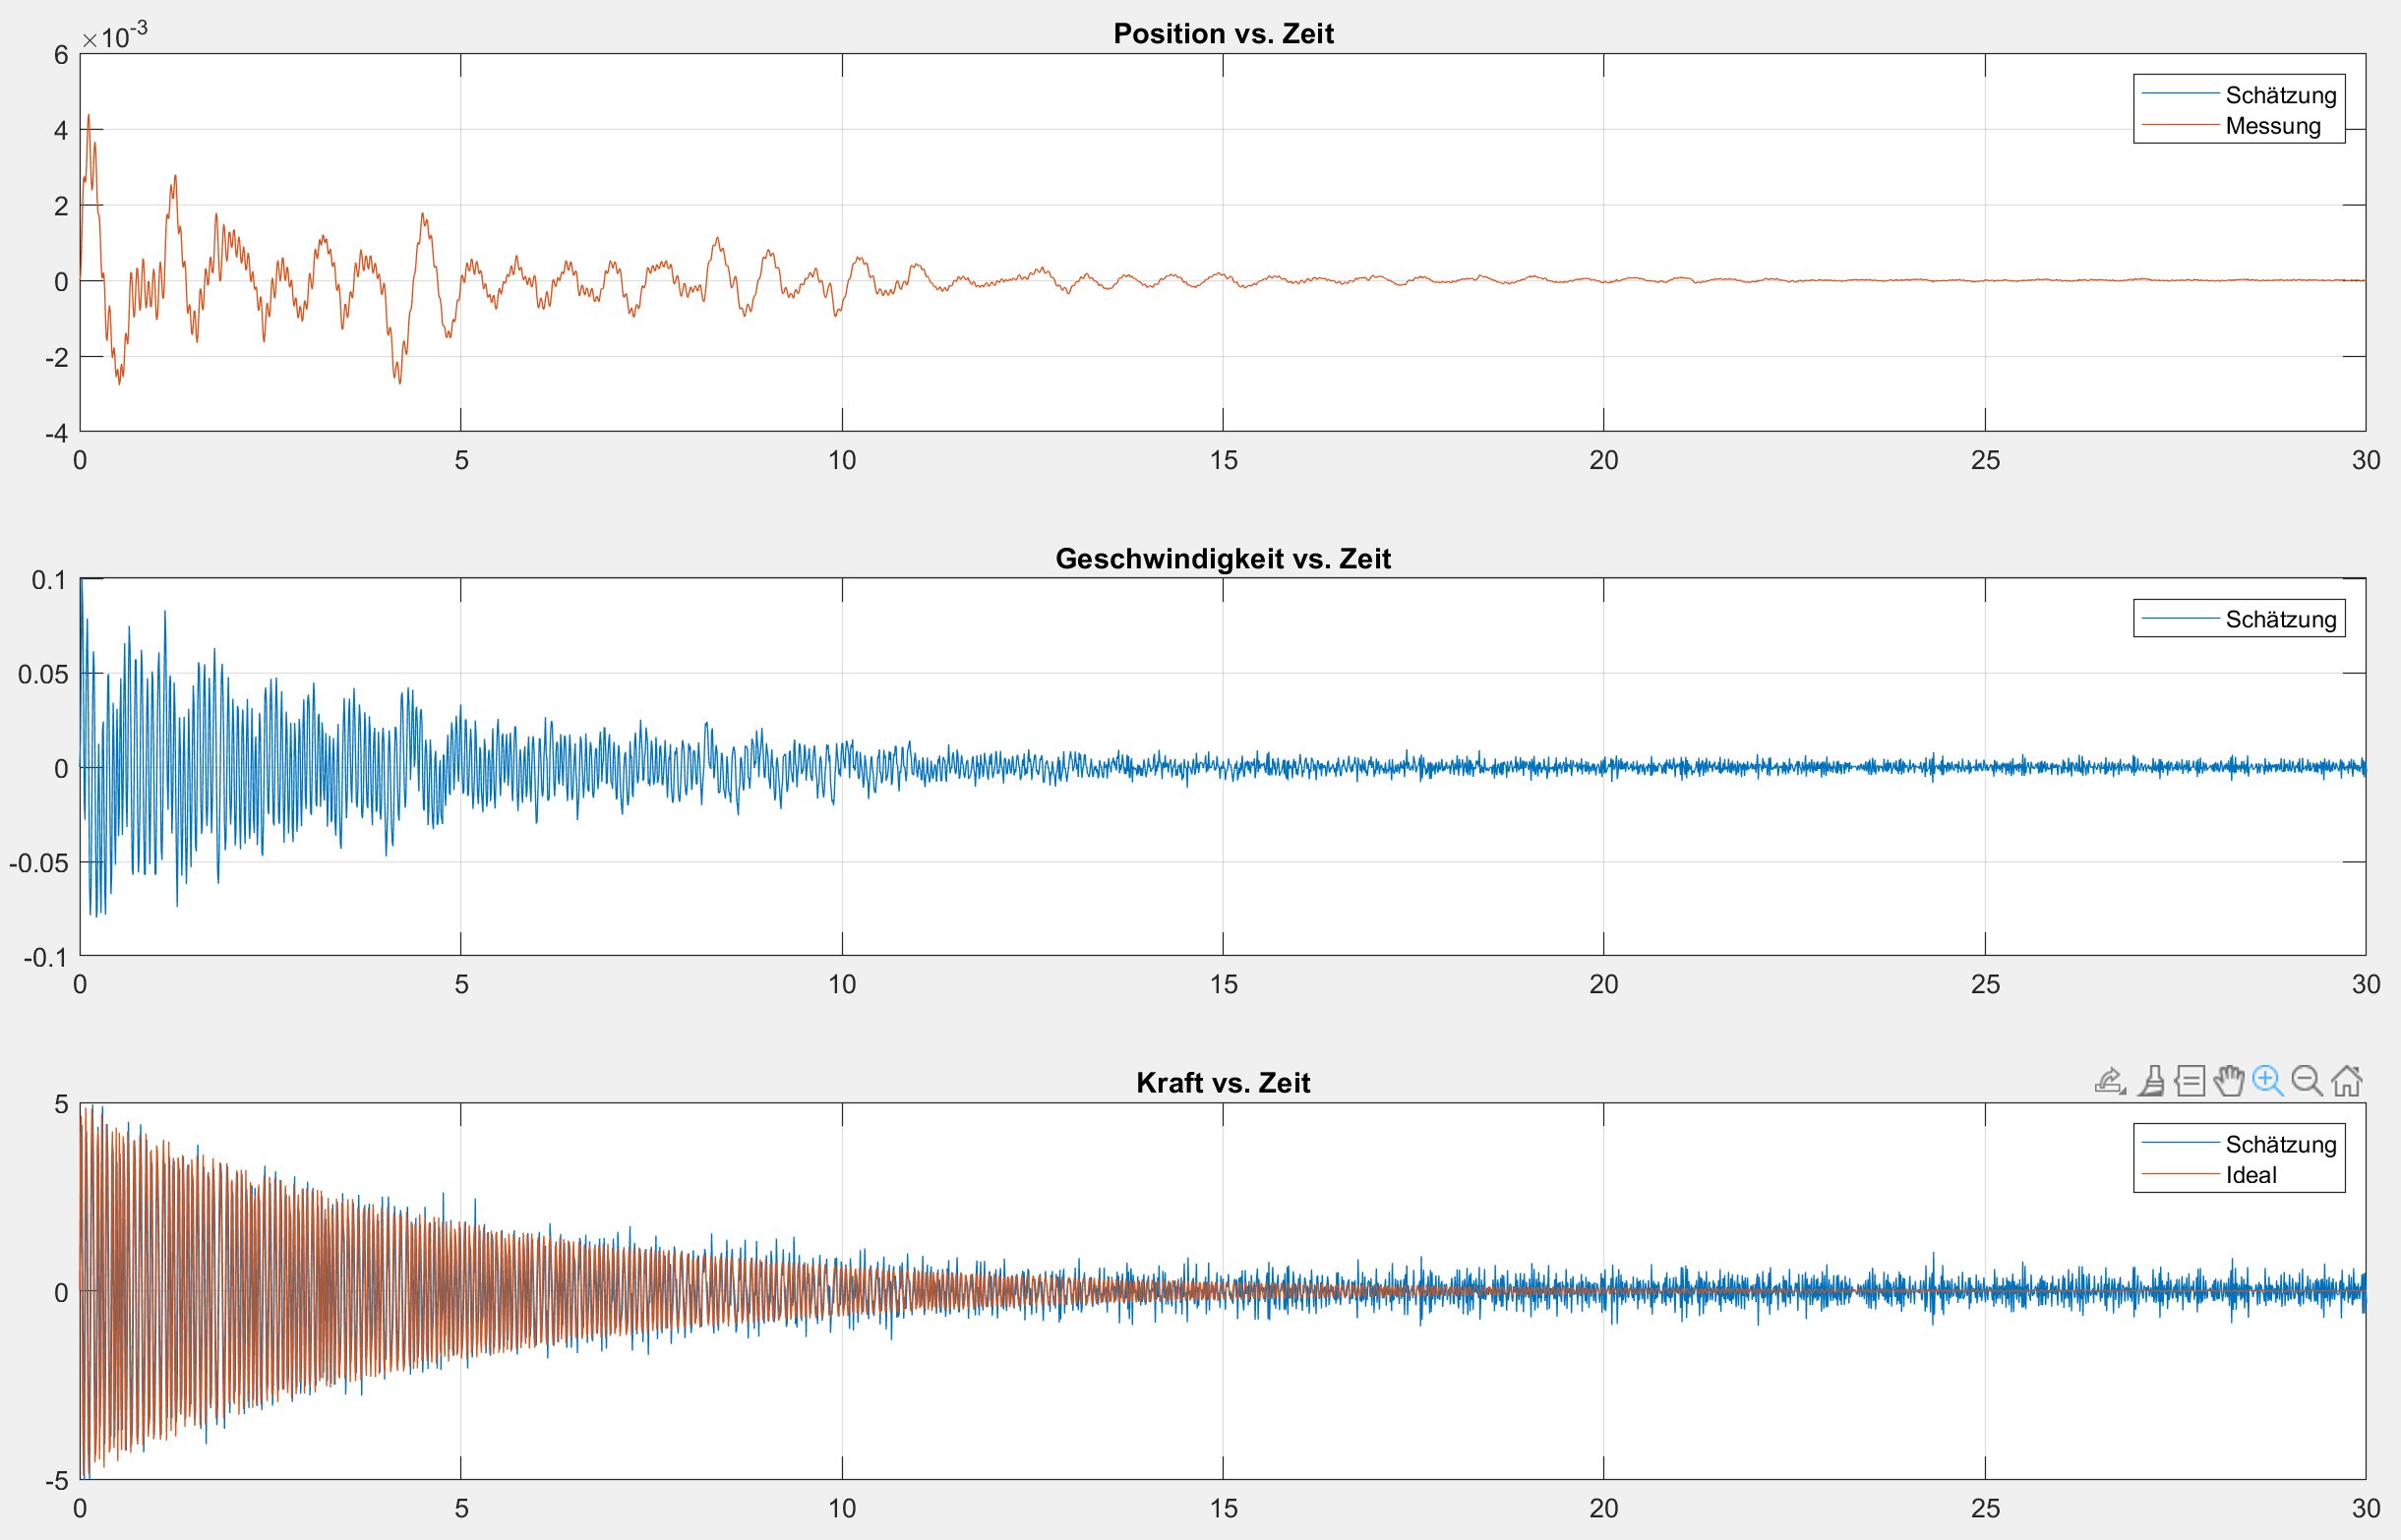
\includegraphics[width=\linewidth,keepaspectratio]{papers/erdbeben/Standard_alles.PNG}
		\caption{Das Position-Zeit-Diagramm zeigt uns die typische Aufzeichnung eines Seismographen während eines Erdbebens. Um die Geschwindigkeit zu erhalten müssen wir die Position einmal ableiten. Ein weiteres Ableiten erzeugt uns die Beschleunigung, respektive die Kraft. Sehr gut ersichtlich ist die Hüllkurve der Amplitude, wie wir sie bei einer gedämpften Schwingung erwarten.}
    \label{erdbeben:fig:standard-alles}
	\end{center}
\end{figure}

\begin{figure}
	\begin{center}
		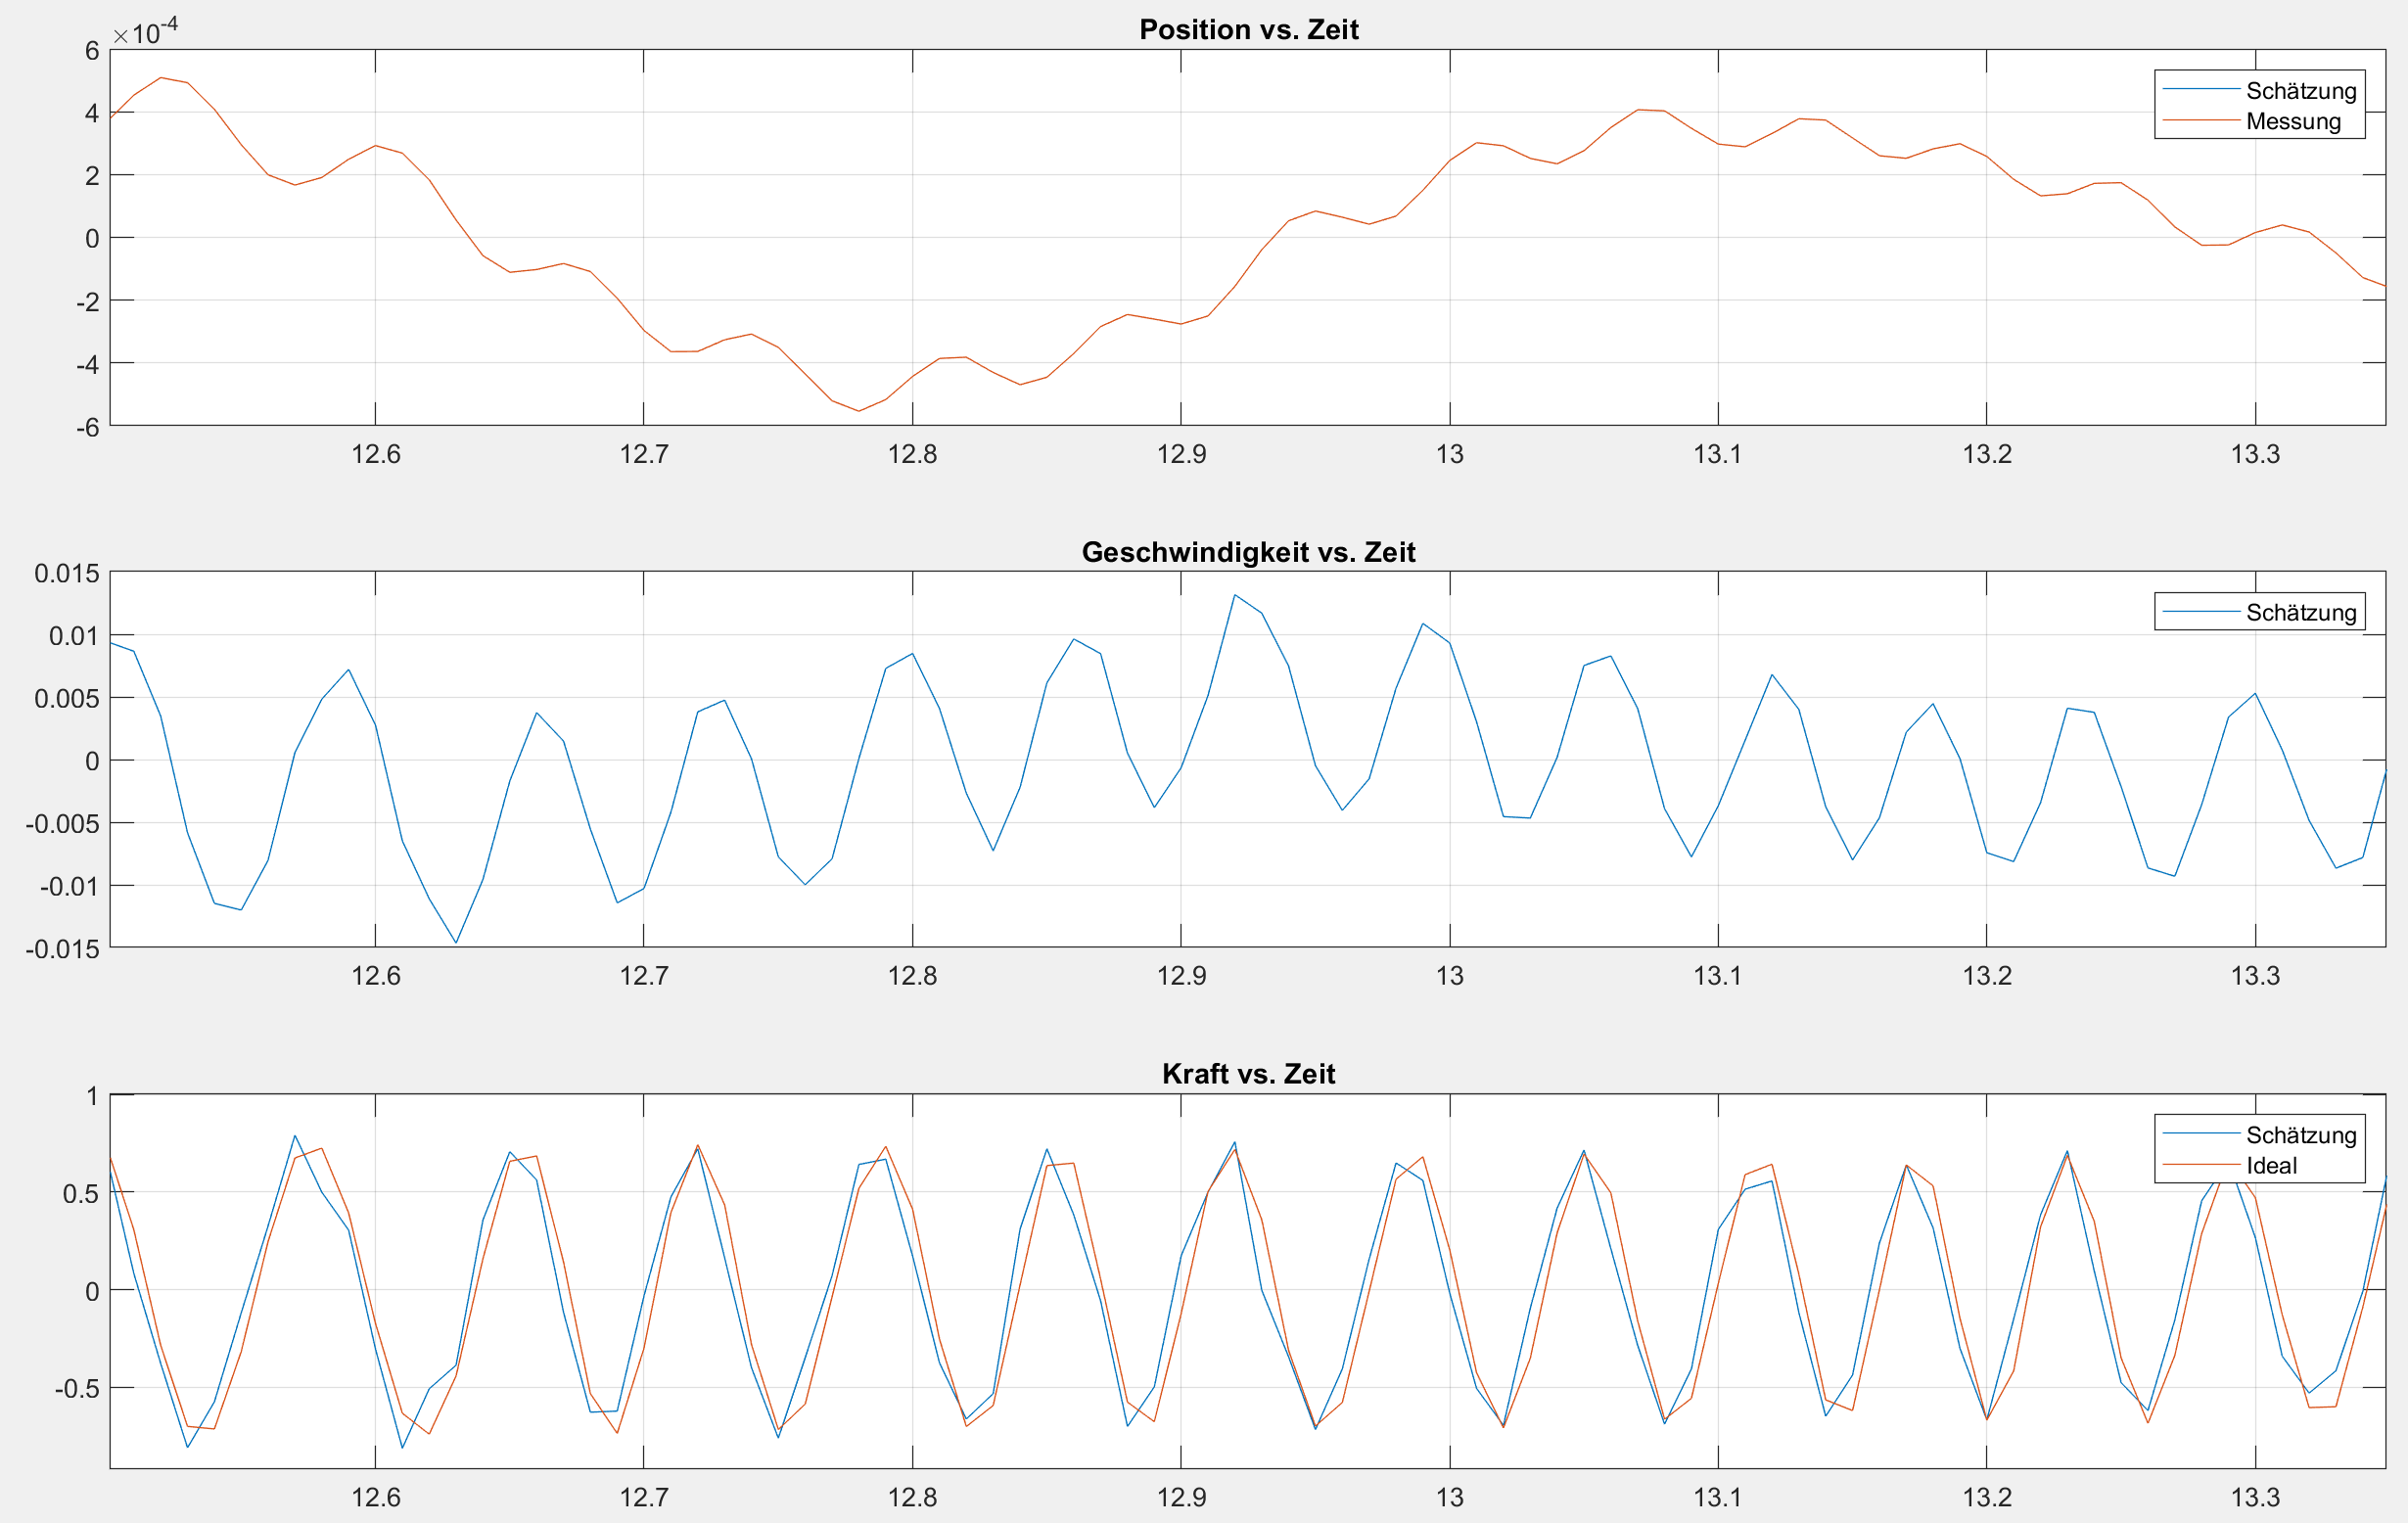
\includegraphics[width=\linewidth,keepaspectratio]{papers/erdbeben/Standard_Zoom.PNG}
		\caption{Erst das Vergrössern an die Datenpunkte zeigt uns auf, wie gut die Schätzung des Kalman-Filters funktioniert.}
    \label{erdbeben:fig:standard-zoom}
	\end{center}
\end{figure}

\subsection{Veränderung der Systemparameter}
Was wir nun testen möchten, sind die Auswirkungen wenn zum Beispiel der Seismograph andere Systemparameter aufweist.
Wir nehmen an, dass sich im Vergleich zum Standardfall die Masse erhöht, die Federkonstante schwächer und die Federdämpfung doppelt so stark wirkt.
Somit gilt neu
\[
m = 0.05,
\qquad
D = 0.5
\qquad \text{und} \qquad
k = 0.02.
\]

Da wir mit dieser Anpassung die Trägheit des Seismogrammes erhöht haben,
erwarten wir eine langsamere Bewegung der Masse,
das heisst die Frequenz wird kleiner.

Betrachten wir Abbildung~\ref{erdbeben:fig:systemparameter-geaendert},
können wir diese Erwartung bestätigen.
Zudem bemerken wir eine grössere Auslenkung der Position,
die wir mir durch die höhere Energie der Masse und geringeren Rücklenkkraft der Feder erklären können.

\begin{figure}
	\begin{center}
		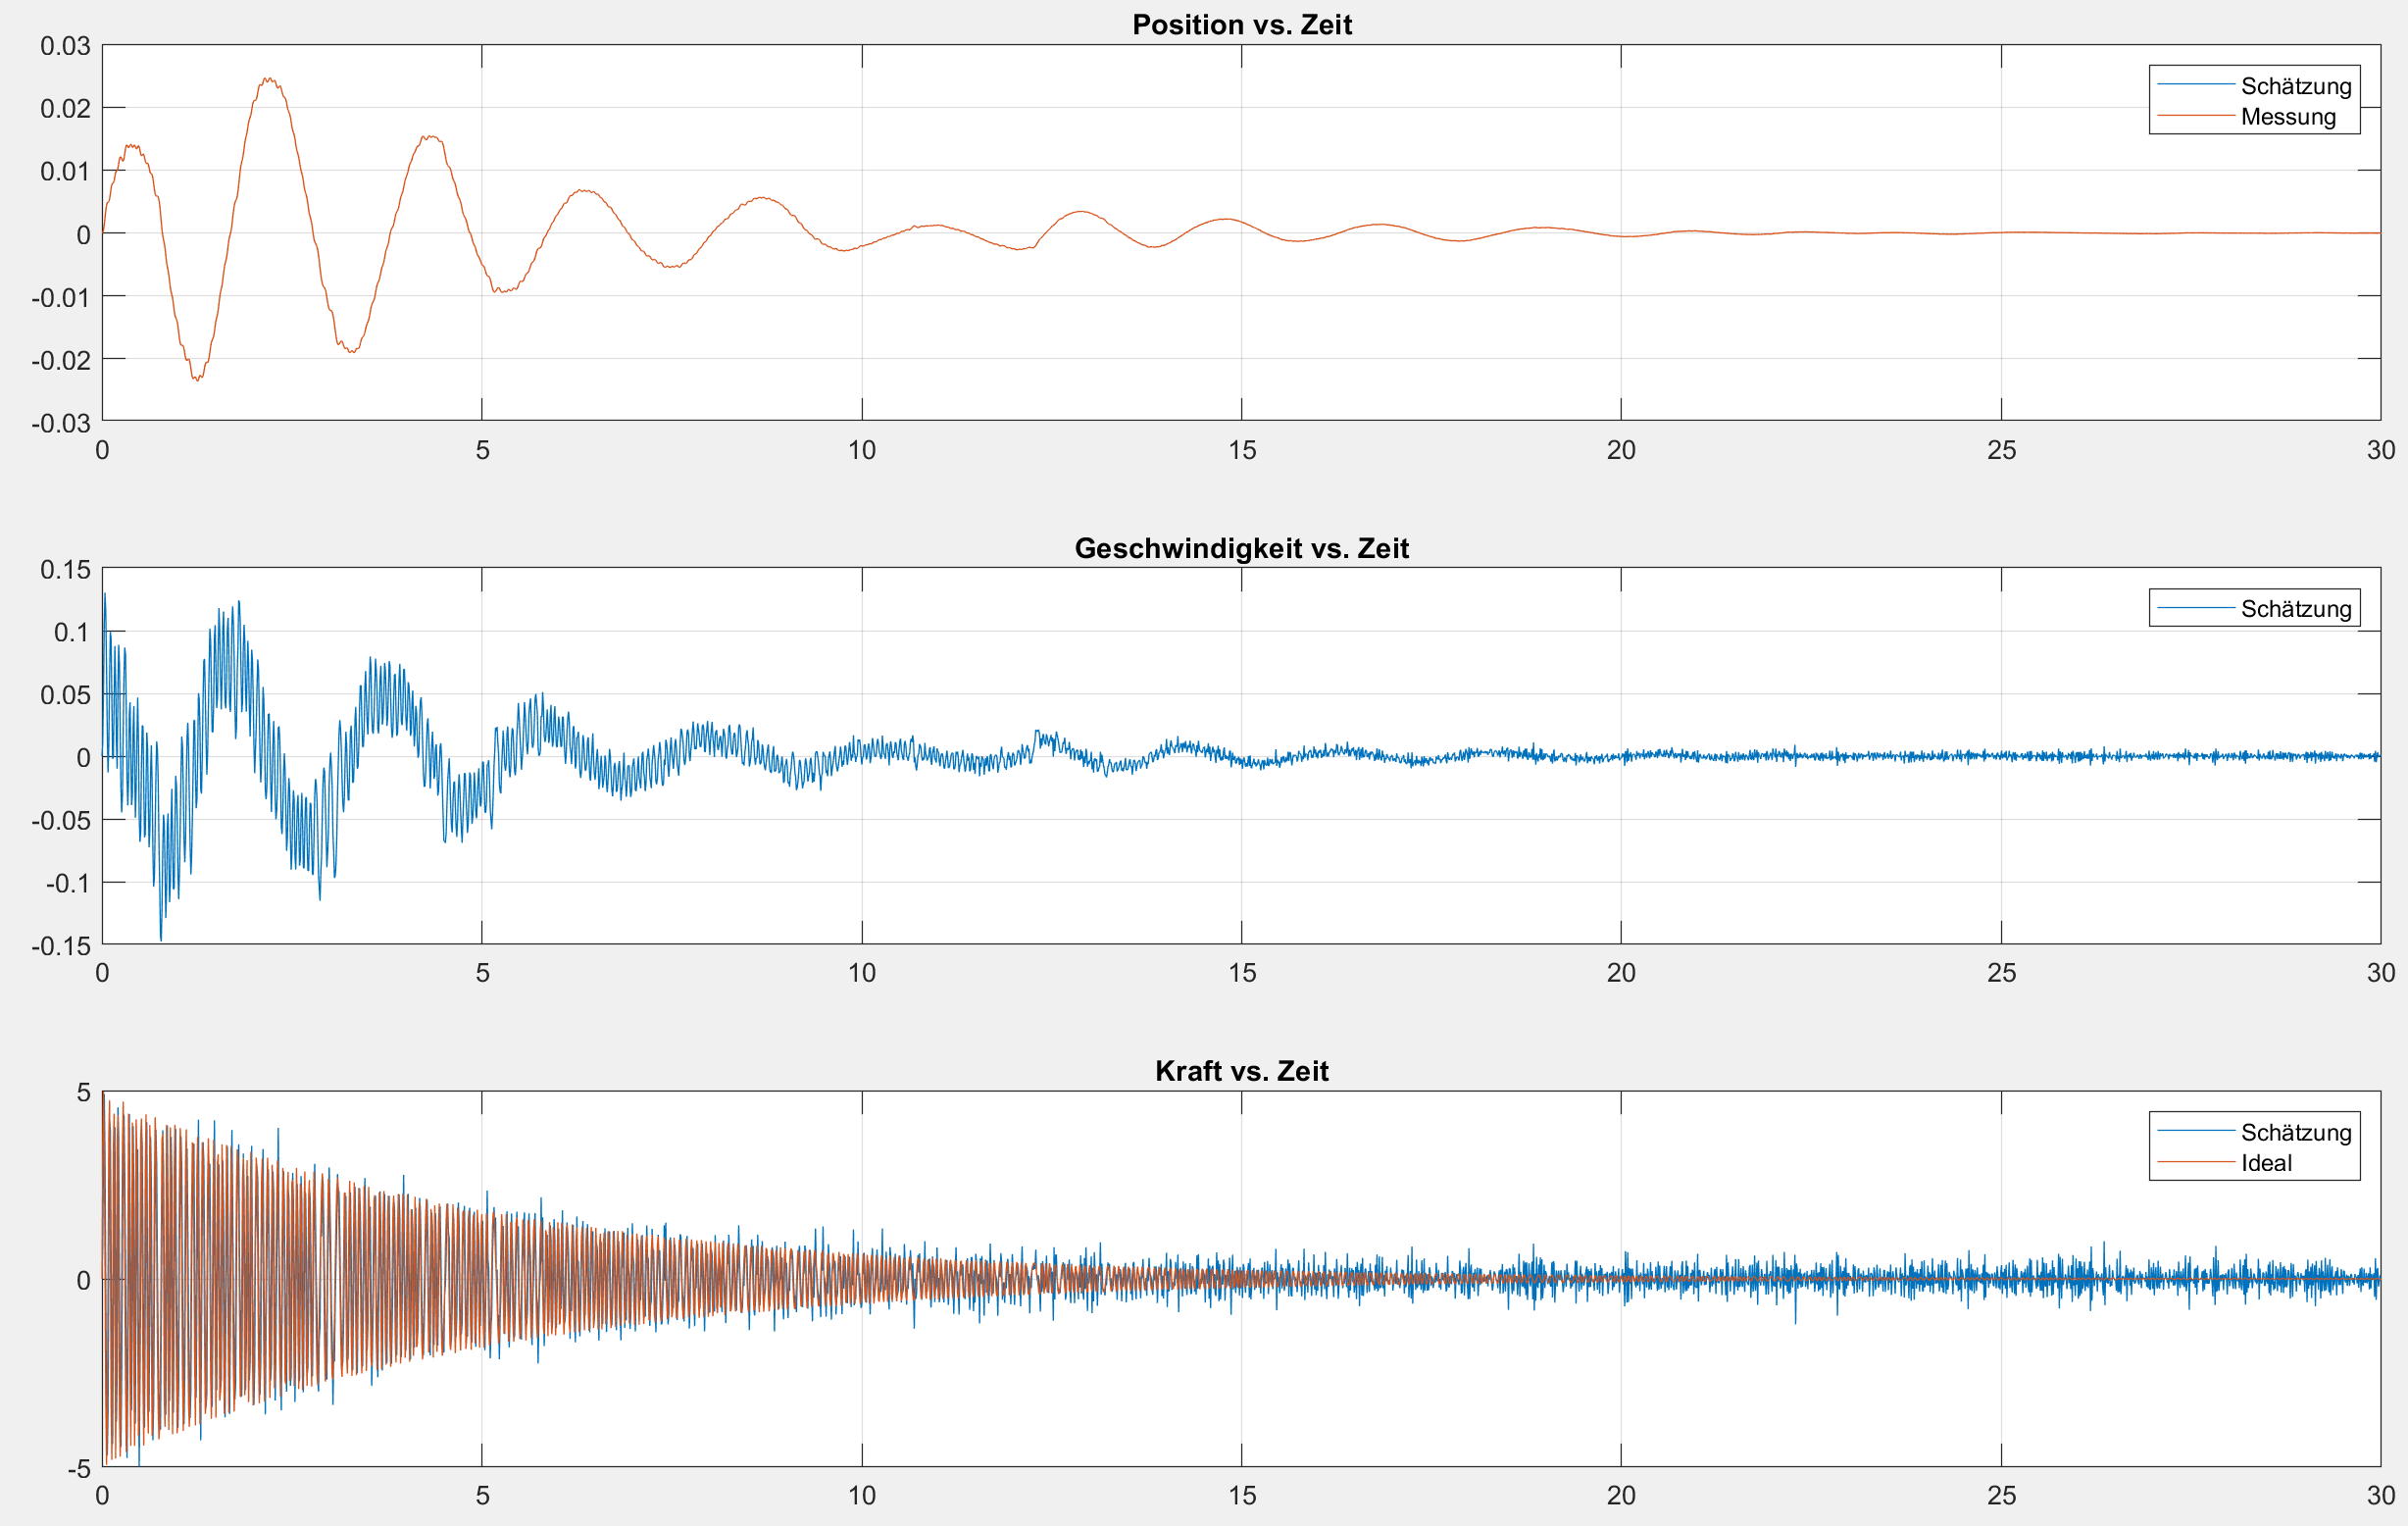
\includegraphics[width=\linewidth,keepaspectratio]{papers/erdbeben/Systemparameter_geaendert_2.PNG}
		\caption{Im Geschwindigkeits-Diagramm erkennen wir, dass sich im Vergleich zum Standardfall, die Auslenkung und Frequenz vergrössert hat. Dies wird mit der Erhöhung der Masse und somit der Trägheit begründet. Auch stellen wir fest, dass die Positionsmessung überwiegend die Eigenfrequenz misst.}
    \label{erdbeben:fig:systemparameter-geaendert}
	\end{center}
\end{figure}


\subsection{Verstärkung des Prozessrauschens}
Falls wir unseren Seismographen in der Nähe einer grösseren Stadt aufstellen, so müssen wir aufgrund der Vibrationen mit einem stärkeren Prozessrauschen rechnen.
Dieses Rauschen beeinflusst die Varianzen der Position und Geschwindigkeit in der Matrix $Q$.
Aus diesem Grund erhöhen wir die Standardabweichungen in der Matrix $Q$ um den Faktor $100$.
Die Auswertung in Abbildung~\ref{erdbeben:fig:prozessrauschen-geaendert} zeigt auf, dass das Kalman-Filter die Schätzung der Kraft nur gering an den Messwerten anpasst.

\begin{figure}
	\begin{center}
		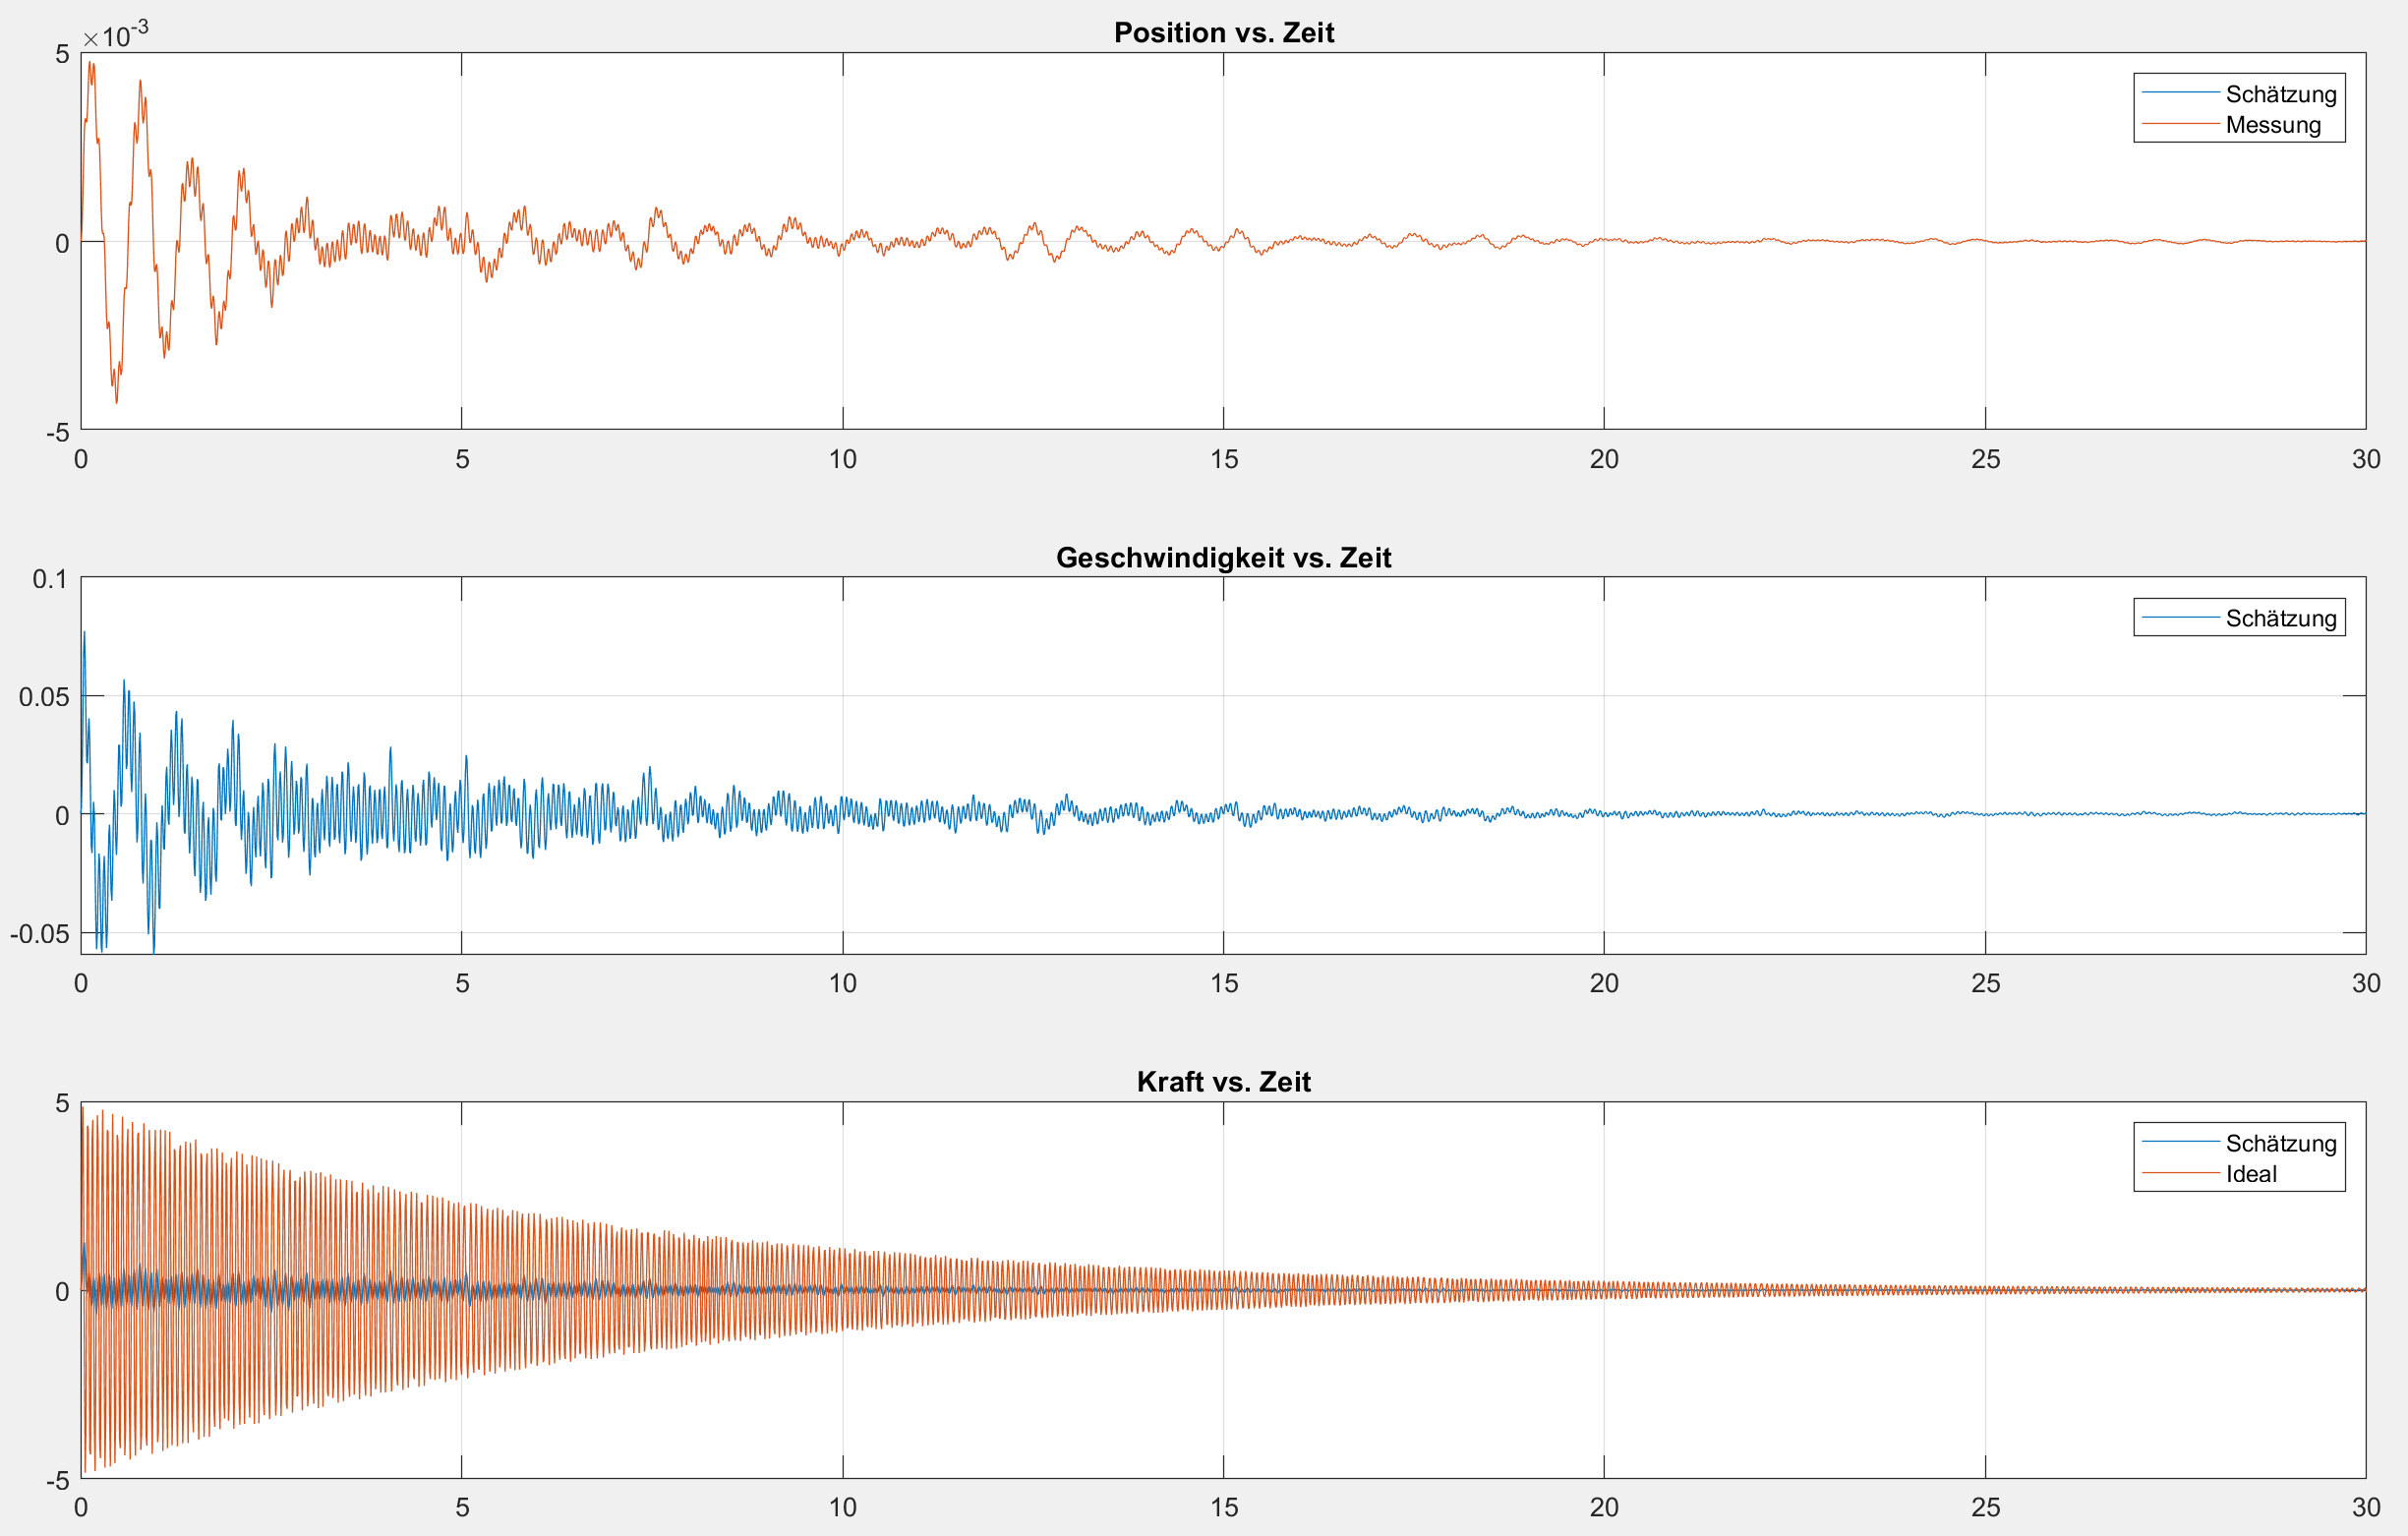
\includegraphics[width=\linewidth,keepaspectratio]{papers/erdbeben/Prozessrauschen_geaendert.PNG}
		\caption{Mit dem Erhöhen des Prozessrauschens gehen wir von einer grösseren Unsicherheit der Systemmatrix aus. Aus diesem Grund folgt das Filter vor allem den Messwerten, was sichtbare Folgen für die Schätzkurve im Kraft-Zeit-Diagramm hat. Hier möchte das Filter auch den Messwerten folgen. Da wir aber für die Kraft keine Messwerte aufzeichnen, erhalten wir eine sehr schwache Kurve}
    \label{erdbeben:fig:prozessrauschen-geaendert}
	\end{center}
\end{figure}

\begin{figure}
	\begin{center}
		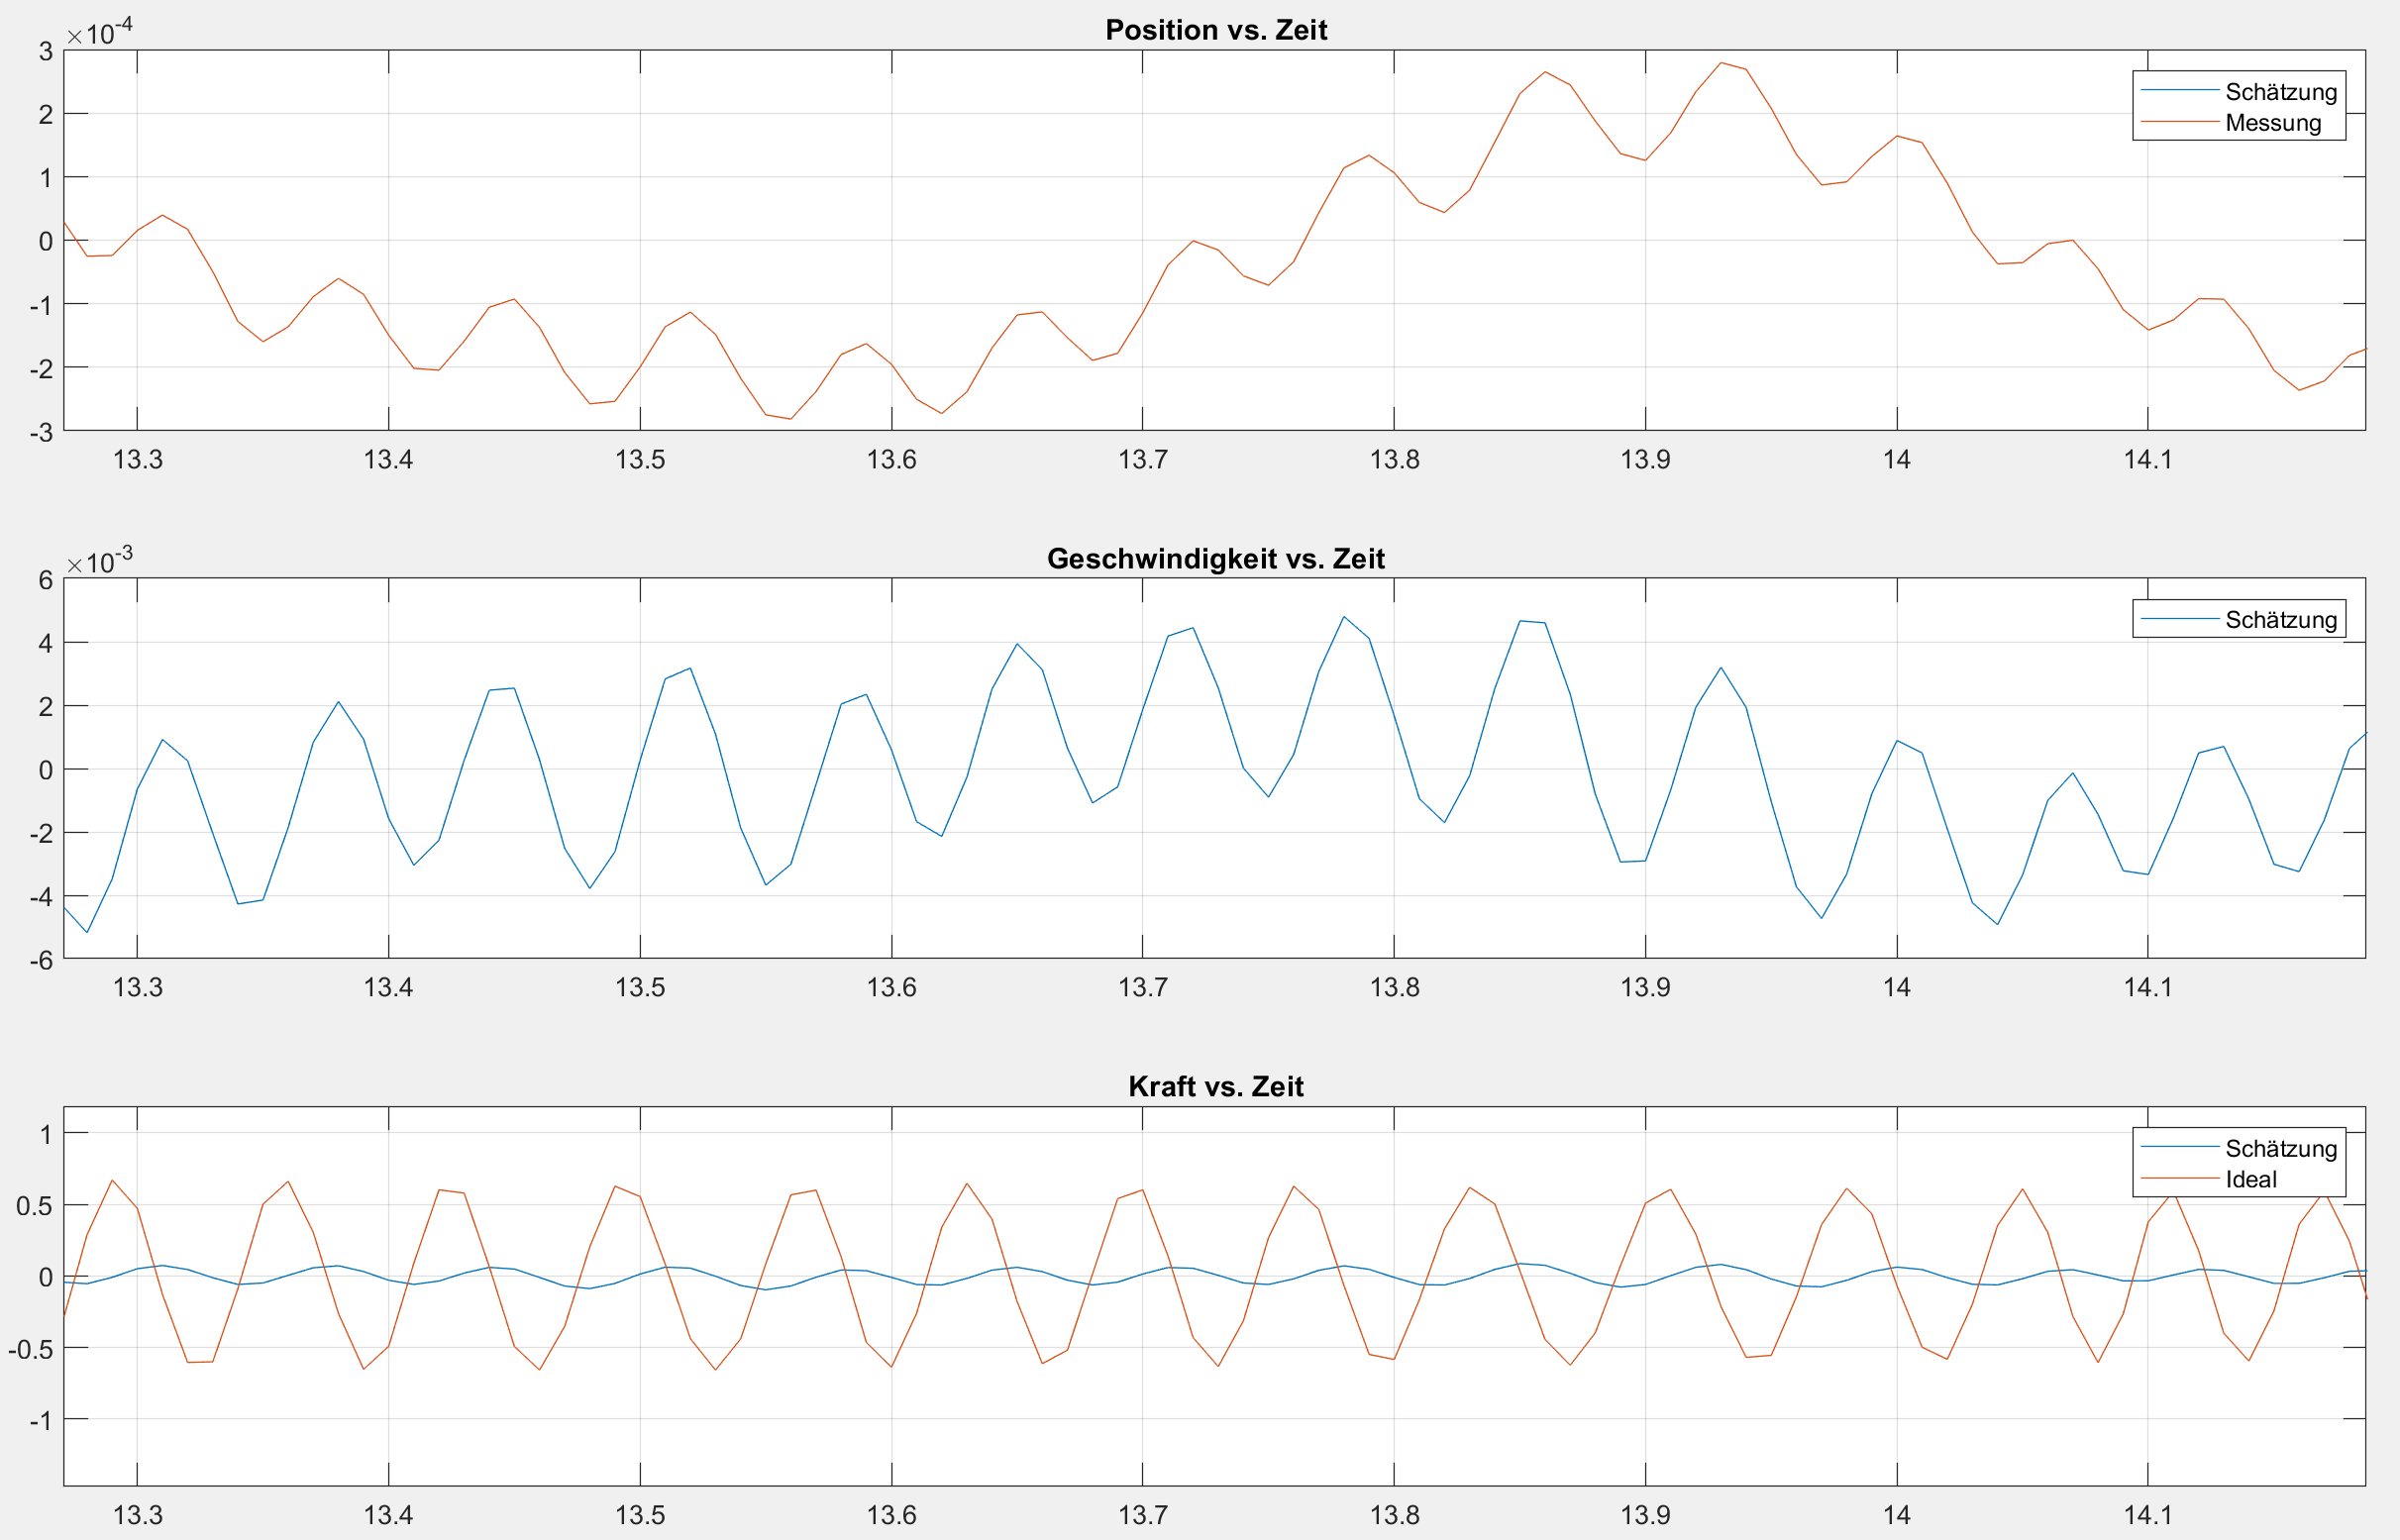
\includegraphics[width=\linewidth,keepaspectratio]{papers/erdbeben/Prozessrauschen_geaendert_zoom.PNG}
		\caption{Die Position kann immernoch präzise geschätzt werden und die Ableitung zur Geschwindigkeit ergibt gute Resultate. Jedoch ist die Schätzkurve der Kraft sehr weit von der idealen Kurve entfernt und nicht nutzbar.}
		\label{erdbeben:fig:prozessrauschen-geaendert-zoom}
	\end{center}
\end{figure}

\subsection{Verstärkung des Messrauschens}
Als letztes verstärken wir das Messrauschen um den Faktor $100$ und belassen wieder den Rest wie im Standardfall.
Wie man eigentlich schon erwarten kann, zeigt uns die Abbildung~\ref{erdbeben:fig:messrauschen-geaendert}, dass das Signal des Messsensors vom Messrauschen gestört wird.
Weil die Messung somit ungenau wird, kann das Kalman-Filter nicht mehr genau arbeiten und produziert eine ungenaues Resultat.

\begin{figure}
	\begin{center}
		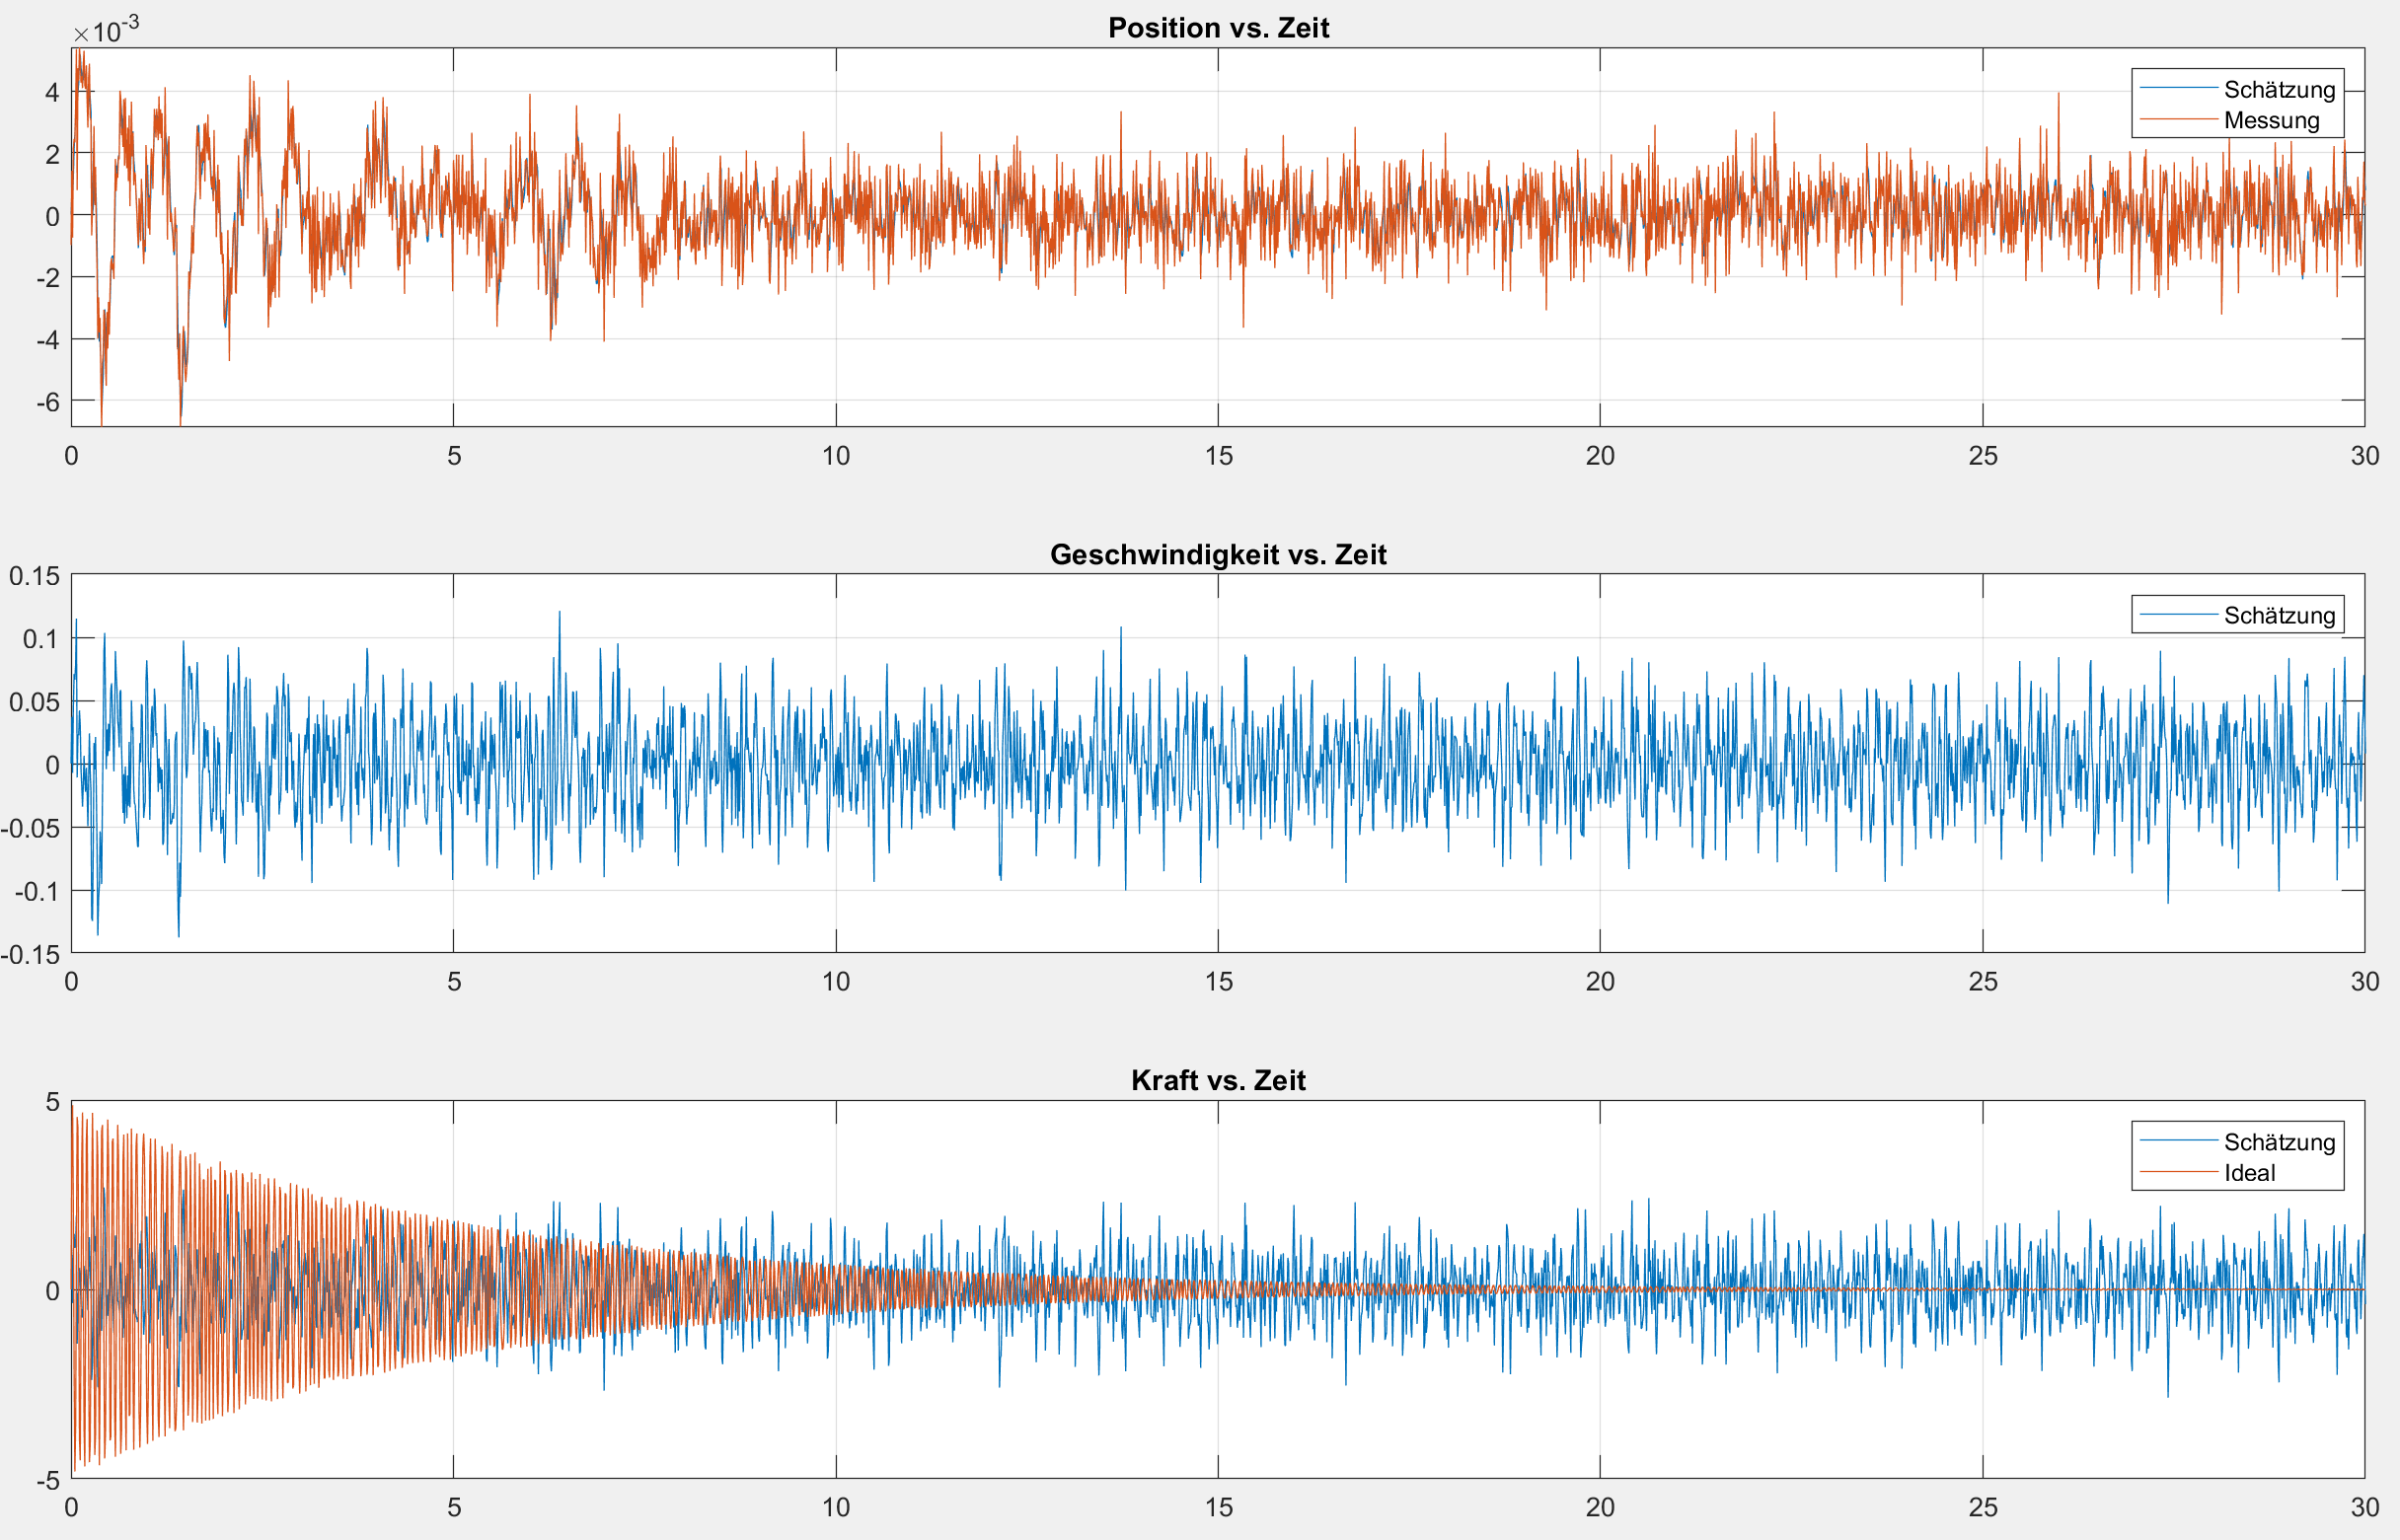
\includegraphics[width=\linewidth,keepaspectratio]{papers/erdbeben/Messrauschen_geaendert.PNG}
		\caption{Im Kraft-Zeit-Diagramm erhalten wir nur bis ca. $t = 10$ gute Schätzwerte. Von $t = 10$ bis $t = 30$ wirkt das Messrauschen zu stark und erhalten keine brauchbaren Werte mehr}
	 \label{erdbeben:fig:messrauschen-geaendert}
	\end{center}
\end{figure}

\begin{figure}
	\begin{center}
		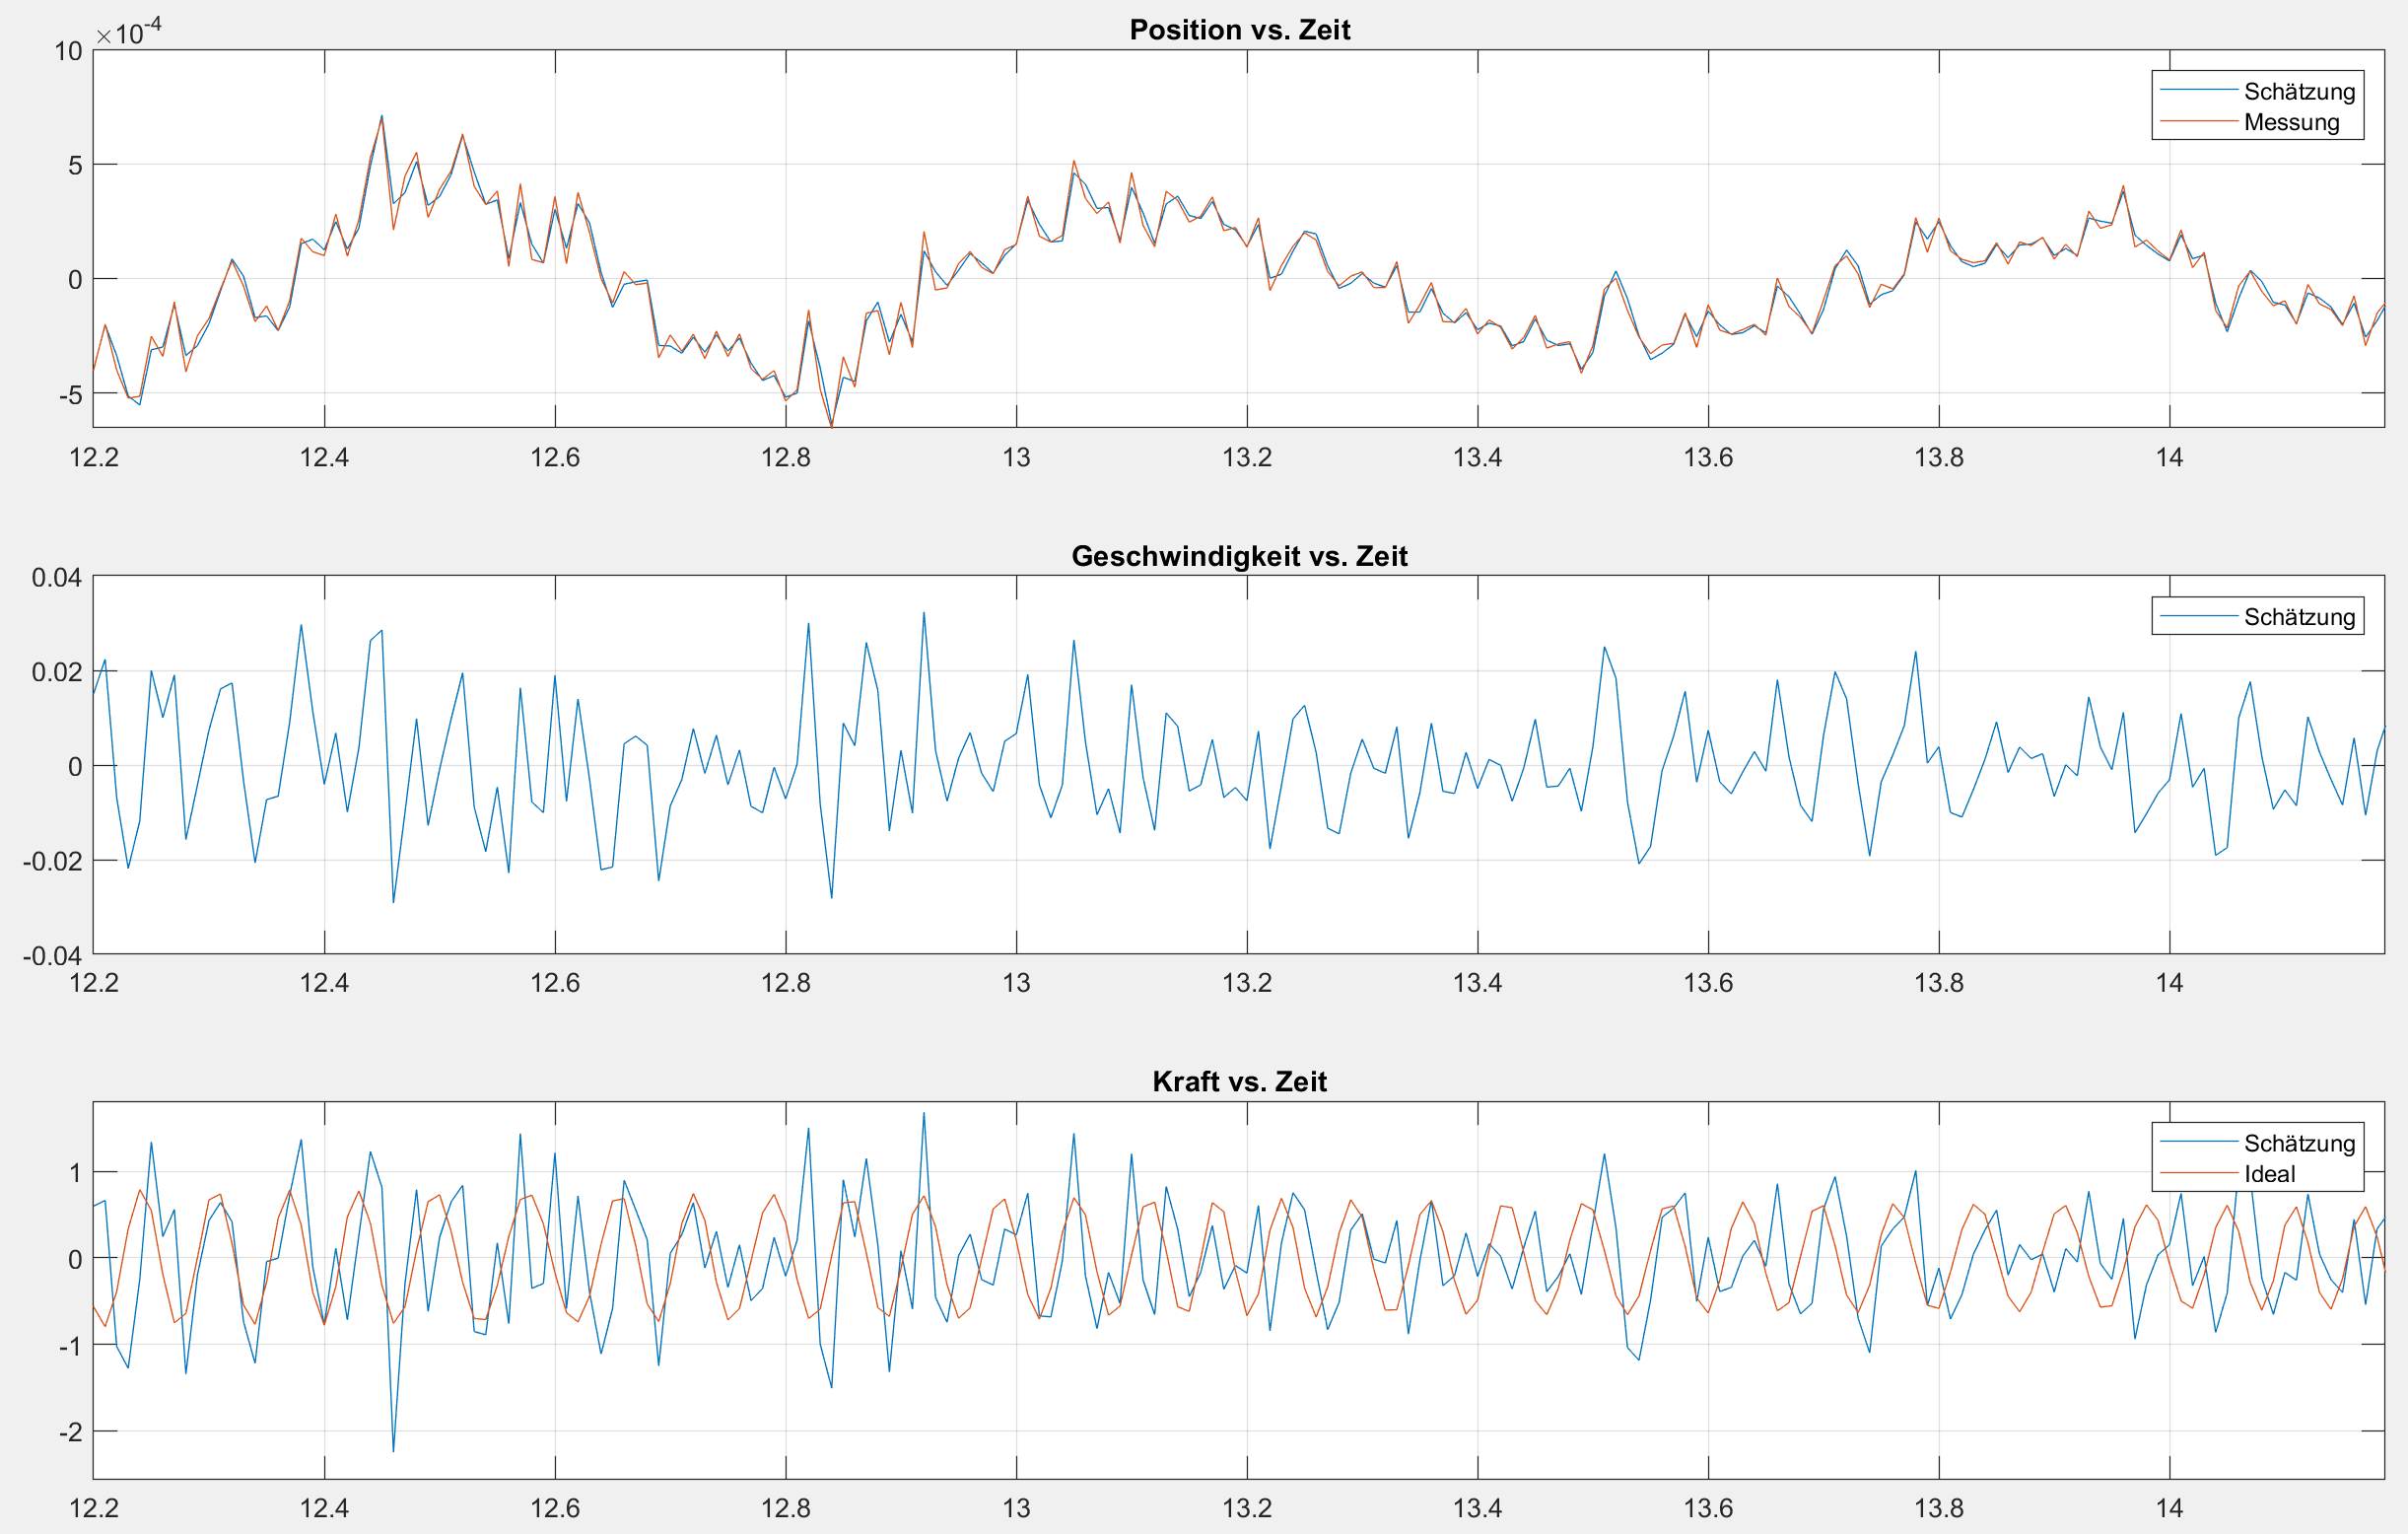
\includegraphics[width=\linewidth,keepaspectratio]{papers/erdbeben/Messrauschen_geaendert_zoom.PNG}
		\caption{Im Position-Zeit-Diagramm erhielten wir bis jetzt immer genaue Schätzungen. Mit einem starken Messrauschen fällt es nun dem Filter schwerer, präzise Werte zu generieren. Die Nahaufnahme im Kraft-Zeit-Diagramm bestätigt uns aber, dass die Messfehler zu gross sind, um ein klares Bild über die äussere Kraft zu erhalten.}
		\label{erdbeben:fig:messrauschen-geaendert_zoom}
	\end{center}
\end{figure}

\subsection{Zusammenfassung}
Wir haben uns zum Ziel gesetzt, die äussere Beschleunigung $a(t)$, bzw. die Kraft $f(t)$ eines Erdbebens zu ermitteln.

Mit der Software Matlab haben wir einen virtuellen Seismographen gebaut und ein künstliches Erdbeben erzeugt.
Der Seismograph war fähig die Position der Masse während der Einwirkung des Erdbebens aufzuzeichnen.
$a(t)$ kann zwar nicht mit Sensoren gemessen werden, jedoch erhalten wir $a(t)$ durch zweifaches Ableiten.
Da wir so aber die innere Beschleunigung erhalten, mussten wir das Kalman-Filter anwenden.
Das Kalman-Filter half uns die äussere Beschleunigung zu schätzen und lieferte erstaunlich genaue Werte.
Ausserdem hat es das Filter geschafft, die Eigenfrequenz der Masse und die Erdbebenfrequenz zu separieren.
Folglich erhielten wir eine Schätzung, die nur das Erdbeben betraf.

Zuletzt haben wir aufgezeigt, das Veränderungen an den System- und Rauschparametern die Genauigkeit und Zuverlässigkeit des Kalman-Filters beeinträchtigen können.

